%%%%%%%%%%%%%%%%%%%%%%%%%%%%%%%%%%%%%%%%%%%%%%%%%%%%%%%%%%%%%%%%%%%%%%%%%%%%%%%%
% Inicializálás                                                                %
%%%%%%%%%%%%%%%%%%%%%%%%%%%%%%%%%%%%%%%%%%%%%%%%%%%%%%%%%%%%%%%%%%%%%%%%%%%%%%%%

%%%%%%%%%%%%%%%%%%%%%%%%%%%%%%%%%%%%%%%%%%%%%%%%%%%%%%%%%%%%%%%%%%%%%%%%%%%%%%%%
% Papírméret, betűméret, margó, magyar karakterek                              %
%%%%%%%%%%%%%%%%%%%%%%%%%%%%%%%%%%%%%%%%%%%%%%%%%%%%%%%%%%%%%%%%%%%%%%%%%%%%%%%%

\documentclass[a4paper,12pt]{article}
\special{papersize=210mm,297mm}

\usepackage{anysize}
\marginsize{2.5cm}{2.5cm}{2.5cm}{2.5cm}

\usepackage[utf8]{inputenc}
\usepackage[magyar]{babel}

%%%%%%%%%%%%%%%%%%%%%%%%%%%%%%%%%%%%%%%%%%%%%%%%%%%%%%%%%%%%%%%%%%%%%%%%%%%%%%%%
% Fedlap inicializálása                                                        %
%%%%%%%%%%%%%%%%%%%%%%%%%%%%%%%%%%%%%%%%%%%%%%%%%%%%%%%%%%%%%%%%%%%%%%%%%%%%%%%%

\usepackage{fedlap}

\csapat{unexpected\_exceptions}{59}
\konzulens{Ferencz Endre}

\taga{Biró Loránd}{NCZAGL}{lol.kylerrr@gmail.com}
\tagb{Kanyó Tibor}{NXWUKE}{kanyo.tibi@gmail.com}
\tagc{Magyar Dániel}{SUFFGT}{samuraidanm@gmail.com}
\tagd{Tarjáni Tamás}{S499KV}{tarjanitomi@gmail.com}
\tage{Vajsz Kornél}{VUYNAW}{roncsipar@gmail.com}

%%%%%%%%%%%%%%%%%%%%%%%%%%%%%%%%%%%%%%%%%%%%%%%%%%%%%%%%%%%%%%%%%%%%%%%%%%%%%%%%
% Fejléc és lábléc                                                             %
%%%%%%%%%%%%%%%%%%%%%%%%%%%%%%%%%%%%%%%%%%%%%%%%%%%%%%%%%%%%%%%%%%%%%%%%%%%%%%%%

\usepackage{fancyhdr}

\setlength{\headheight}{1.4em}
\setlength{\headsep}{2em}

\fancyhf{}
\fancyhead[OL] { \leftmark{} }
\fancyhead[OR] { \tmpcsapat }
\fancyfoot[OC] { \thepage }
\fancyfoot[OR] { \tmpdatum }

\pagestyle{fancy}

%%%%%%%%%%%%%%%%%%%%%%%%%%%%%%%%%%%%%%%%%%%%%%%%%%%%%%%%%%%%%%%%%%%%%%%%%%%%%%%%
% Napló                                                                        %
%%%%%%%%%%%%%%%%%%%%%%%%%%%%%%%%%%%%%%%%%%%%%%%%%%%%%%%%%%%%%%%%%%%%%%%%%%%%%%%%

\usepackage{longtable}

\newenvironment{journal}
{
	\hbadness 10000
	\begin{longtable}{|p{60pt}|l|l|p{216pt}|}
	\hline
	\textbf{Kezdet} & \textbf{Időtartam} & \textbf{Résztvevők} & \textbf{Leírás} \\
	\hline
	\endfirsthead
	\hline
	\textbf{Kezdet} & \textbf{Időtartam} & \textbf{Résztvevők} & \textbf{Leírás} \\
	\hline
	\endhead
}
{
	\end{longtable}
}

\newcommand{\journalentry}[4]
{
	{#1} & {#2} óra & \parbox{50pt}{#3} & {#4} \\
	\hline
}

%%%%%%%%%%%%%%%%%%%%%%%%%%%%%%%%%%%%%%%%%%%%%%%%%%%%%%%%%%%%%%%%%%%%%%%%%%%%%%%%
% UseCase leírás                                                               %
%%%%%%%%%%%%%%%%%%%%%%%%%%%%%%%%%%%%%%%%%%%%%%%%%%%%%%%%%%%%%%%%%%%%%%%%%%%%%%%%

\newenvironment{usecase}
{
	\hbadness 10000
	\begin{longtable}[l]{|p{100pt}|p{328pt}|}
	\hline
	\endfirsthead
	\hline
	\endhead
}
{
	\hline
	\end{longtable}
}

\newcommand{\usecaseentry}[2]
{
	\hline
	\textbf{#1} & {#2}\\
}

%%%%%%%%%%%%%%%%%%%%%%%%%%%%%%%%%%%%%%%%%%%%%%%%%%%%%%%%%%%%%%%%%%%%%%%%%%%%%%%%
% FileList leírás                                                               %
%%%%%%%%%%%%%%%%%%%%%%%%%%%%%%%%%%%%%%%%%%%%%%%%%%%%%%%%%%%%%%%%%%%%%%%%%%%%%%%%

\newenvironment{filelist}
{
	\hbadness 10000

	\begin{longtable}{|p{145pt}|p{35pt}|p{63pt}|p{163pt}|}
	\hline
	\textbf{Fájl neve} & \textbf{Méret} & \textbf{Keletkezés ideje} & \textbf{Tartalom} \\
	\hline
	\endfirsthead
	\hline
	\textbf{Fájl neve} & \textbf{Méret} & \textbf{Keletkezés ideje} & \textbf{Tartalom} \\
	\hline
	\endhead
}
{
	\end{longtable}
}

\newcommand{\filelistentry}[4]
{
	{#1} & {#2} b & {#3} & {#4} \\
	\hline
}
%%%%%%%%%%%%%%%%%%%%%%%%%%%%%%%%%%%%%%%%%%%%%%%%%%%%%%%%%%%%%%%%%%%%%%%%%%%%%%%%
% Egyebek                                                                      %
%%%%%%%%%%%%%%%%%%%%%%%%%%%%%%%%%%%%%%%%%%%%%%%%%%%%%%%%%%%%%%%%%%%%%%%%%%%%%%%%

\usepackage{graphicx}		% Kepek beillesztesehez
\usepackage{epstopdf}		% EPS fajlok felismeresehez
\graphicspath{{Images/}}	% Az Images mappaban keresse a kepeket

\anyag{3. Analízis modell kidolgozása}
\datum{2012. február 26.}
\setcounter{section}{2}

%%%%%%%%%%%%%%%%%%%%%%%%%%%%%%%%%%%%%%%%%%%%%%%%%%%%%%%%%%%%%%%%%%%%%%%%%%%%%%%%
% Dokumentum                                                                   %
%%%%%%%%%%%%%%%%%%%%%%%%%%%%%%%%%%%%%%%%%%%%%%%%%%%%%%%%%%%%%%%%%%%%%%%%%%%%%%%%

\begin{document}

\fedlap

\section{Analízis modell kidolgozása}

\subsection{Objektum katalógus}

\subsubsection{Model package}

\textbf{LevelDescriptor}: Egy-egy pálya leírását tartalmazza. Tárolja a pályaelemek leírásait, a kulcsok, ajtók és kezdőpont helyzeteit. Ezen osztály kezeli saját maga beolvasását fájlból.

\textbf{LevelPartDescriptor}: Egy pályaelem paramétereit tárolja: hol van a pályán belül és hogy az egyes blokkok (faldarabok) hol találhatók benne.

\textbf{BlockDescriptor}: Magát a faldarabot, egy blokkot, leíró osztály, melynek van pozíciója és mérete a síkban.

\textbf{LevelObjectDescriptor}: Ezen osztály tárolja minden objektum (kezdő, kulcs, ajtó) típus adatait: milyen fajta típusú az adott objektum, melyik pályaelemen van és azon belül is hol.

\textbf{LevelObjectType}: A pályán elhelyezhető objektumok típusainak felsorolása. Jelen esetben ezek: kezdési pont, kulcs és ajtó.

\subsubsection{GameLogic package}

\textbf{Rectangle}: Egy téglalap alakzatot reprezentáló osztály. Rendelkezik valós pozícióval és mérettel, valamint képes eldönteni, hogy egy másik Rectangle osztállyal érintkezik-e és hogy egy adott pont benne van-e.

\textbf{GameObject}: Ezek a játékban szereplő objektumok. Tartalmazza, hogy melyik pályaelemben található az adott objektum, illetve hogy azon belül hol található, ezt az őt magába foglaló téglalap pozíciója segítségével tárolja. Továbbá képes meghatározni, hogy érintkezik-e másik játékban szereplő objektummal.

\textbf{LevelPart}: Egy pályaelemet reprezentáló osztály. Tárolja az adott pályaelemhez tartozó blokkokat, valamint azt, hogy melyik pályaelemekkel szomszédos és hogy hova lehet átmenni róla.

\textbf{Level}: Ez a fő vezérlő osztály az egész játéklogikában. Tárolja azokat pályaelemet, amikből az adott pálya áll, továbbá ő intézi a pályaelemek tili-toli csúsztatását és a játék állapotának figyelését (teljesítettük-e már).

\textbf{Block}: Egy faldarabot jelképező játék objektum. 

\textbf{KeyHolder}: Egy kulcs helyét jelző játék objektum, azt tárolja van-e ott még kulcs.

\textbf{Door}: Egy üres GameObject osztály, mely csak azt reprezentálja, hogy helyileg hova kell menni a pálcikaemberrel, amennyiben megszereztük az összes kulcsot a pályán.

\textbf{Player}: A játékost reprezentáló játékobjektum, a játékos mozgását vezérli az inputok alapján.

\textbf{Direction}: Egy felsorolás amivel irányt jelezhetünk, többek között a pályaelemek csúsztatásának irányát adhatjuk meg vele.

\subsection{Osztályok leírása}

Az osztályok leírása során, amely osztálynál nem szerepel egy-egy tulajdonság, például \textbf{Ősosztály} vagy \textbf{Interfész}, az értelemszerűen azt jelöli, hogy az adott osztály nem rendelkezik vele.

\subsubsection{LevelDescriptor}
	\begin{description}
		\item[Felelősség] \hfill \\
		Egy pálya felépítéséhez szükséges leíró információkat tárolja. A mérete legalább 1x2 vagy 2x1 kell hogy legyen.
		
		\item[Attribútumok]\hfill \\
		\textbf{\emph{int Width}}: pályaelemek száma egy sorban
		
		\textbf{\emph{int Height}}: pályaelemek száma egy oszlopban
		
		\textbf{\emph{LevelPartDescriptor[] Parts}}: az adott pályához tartozó pályaelemek listája
		
		\textbf{\emph{LevelObjectDescriptor}}: a pályán szereplő minden objektumot tartalmazó lista
				
		\item[Metódusok]\hfill \\
		\textbf{\emph{LevelDescriptor load(string)}}: betölti a megadott fájlból a pálya leíró objektumot.
						
	\end{description}

\subsubsection{LevelPartDescriptor}
	\begin{description}
		\item[Felelősség] \hfill \\
		Egy adott pályaelem szerkezetének leírását tartalmazza. A pozíció egész értékű, a bal-felső elem koordinátája 0;0. A közbefogott tér 10x10-es méretű, minden benne lévő pozíció diszkrét értékű.
		
		\item[Attribútumok]\hfill \\
		\textbf{\emph{int X}}: az adott pályaelem pályán belüli hollétének x koordinátája
		
		\textbf{\emph{int Y}}: az adott pályaelem pályán belüli hollétének y koordinátája
		
		\textbf{\emph{BlockDescriptor[] Blocks}}: a pályaelem kialakítását meghatározó blokkok listája
	\end{description}
	
\subsubsection{BlockDescriptor}
	\begin{description}
		\item[Felelősség] \hfill \\
		Egy pályaelem kialakítását szolgáló blokk leírását tartalmazza.
				
		\item[Attribútumok]\hfill \\
		\textbf{\emph{int X}}: az adott blokk x koordinátája a pályaelemben
		
		\textbf{\emph{int Y}}: az adott blokk y koordinátája a pályaelemben
		
		\textbf{\emph{int Width}}: a blokk szélessége
		
		\textbf{\emph{int Height}}: a blokk magassága
						
	\end{description}

\subsubsection{LevelObjectDescriptor}
	\begin{description}
		\item[Felelősség] \hfill \\
		A pályán szereplő objektumok leírója.
		
		\item[Attribútumok]\hfill \\
		\textbf{\emph{int X}}: az adott objektum a pályaelemen való hollétének x koordinátája
		
		\textbf{\emph{int Y}}: az adott objektum pályaelemen való hollétének y koordinátája
		
		\textbf{\emph{int LevelPartIndex}}: a tartalmazó pályaelem indexe
		
		\textbf{\emph{LevelObjectType Type}}: az objektum típusa
						
	\end{description}

\subsubsection{LevelObjectType}
	\begin{description}
		\item[Felelősség] \hfill \\
		A pályán elhelyezhető objektumok típusainak felsorolása. A lehetséges értékek: Key, Door, Spawn.
		
	\end{description}

\subsubsection{Rectangle}
	\begin{description}
		\item[Felelősség] \hfill \\
		Egy téglalap alakzatot reprezentáló osztály. Ismeri a pozícióját és méretét, illetve tudja, hogy metszi-e egy másik ugyanilyen típusú objektum és hogy egy adott pont benne van-e. Minden GameObject helyét és méreteit az őt tartalmazó Rectangle segítségével adjuk meg. Egyfajta hitboxként is funkcionál.
				
		\item[Attribútumok]\hfill \\
		\textbf{\emph{float X}}: a téglalap x koordinátája
		
		\textbf{\emph{float Y}}: a téglalap y koordinátája
		
		\textbf{\emph{float Width}}: a téglalap szélessége
		
		\textbf{\emph{float Height}}: a téglalap magassága
		
		\item[Metódusok]\hfill \\
		\textbf{\emph{bool Intersects(Rectangle other)}}: eldönti, hogy a paraméterül kapott másik Rectangle-lel metszik-e egymást
		
		\textbf{\emph{bool Contains(float x, float y)}}: egy (x,y) koordinátájú pontról megmondja, hogy a téglalap területén van-e
						
	\end{description}

\subsubsection{GameObject}
	\begin{description}
		\item[Felelősség] \hfill \\
		Minden, a pályaelemekben található objektum (Block, KeyHolder, Door, Player) ebből az absztrakt osztályból származik. Egy Rectangle osztály segítségével tárolja a méretét és helyét, illetve tudja, hogy melyik pályaelemben található. A tárolt Rectangle objektum Intersects metódusára építve végzi az ütközésdetekciót. A GameObject meguk frissítik a pozíciójukat.
		
		\item[Attribútumok]\hfill \\
		\textbf{\emph{LevelPart LevelPart}}: referencia arra a pályaelemre, amelyikben van
		
		\textbf{\emph{Rectangle Location}}: egy Rectangle objektum, a pozíció és méret tárolásához
		
		\item[Metódusok]\hfill \\
		\textbf{\emph{bool CollidesWith(GameObject other)}}: ütközésdetektáló metódus. A Rectangle Intersects függvényétől annyiban különbözik, hogy azt is vizsgálja, hogy a két vizsgált objektum egy pályaelemben található-e (vagyis ténylegesen metszik-e egymást).
						
	\end{description}

\subsubsection{LevelPart}
	\begin{description}
		\item[Felelősség] \hfill \\
		Egy pályaelemet reprezentáló osztály. Tárolja a helyét a pályán belül, a benne előforduló blokkokat, a szomszédos pályaelemeket, illetve, hogy ezek közül melyikbe lehet átmenni.

		\item[Attribútumok]\hfill \\		
		\textbf{\emph{int X}}: a pályaelem X irányú pozíciója
		
		\textbf{\emph{int Y}}: a pályaelem Y irányú pozíciója
		
		\textbf{\emph{Block[] Blocks}}: a pályaelemben szereplő blokkok
		
		\textbf{\emph{LevelPart[] Neighbours}}: a szomszédos pályaelemeket tároló Direction szerint címezhető tábla.
		
		\textbf{\emph{bool[] Passabilities}}: a különböző irányokba való átjárhatóságot tároló Direction szerint címezhető tábla.
		
		\item[Metódusok]\hfill \\
		\textbf{\emph{void Update()}}: újraszámolja a Neighbours és a Passabilities listákat
	\end{description}
	
\subsubsection{Level}
	\begin{description}
		\item[Felelősség] \hfill \\
		Ez a fő vezérlő osztály az egész játéklogikában. Ő hozza létre a játékos, az ajtó, a kulcs helyek, a pályát alkotó pályaelemeket vezérlő osztályokat. Ez az osztály végzi a játék állapotának frissítését és a pályaelemek tili-toli módú irányítását is.
		
		\item[Attribútumok]\hfill \\
		\textbf{\emph{int Width}}: a pálya szélessége
		
		\textbf{\emph{int Height}}: a pálya magassága
		
		\textbf{\emph{LevelPart[] Parts}}: a pályát alkotó pályaelemek listája
		
		\textbf{\emph{KeyHolder[] KeyHolders}}: mindezon helyek a pályán, ahol van/volt kulcs
		
		\textbf{\emph{Door Door}}: a pálya végét jelképező ajtó
		
		\textbf{\emph{bool isCompleted}}: ez az attribútum jelzi a pálya állapotát.
		
		\textbf{\emph{Player Player}}: a játékost leíró Player objektum
		
		\item[Metódusok]\hfill \\
		\textbf{\emph{void Update()}}: megvizsgálja a Player aktuális pozícióját és frissíti a pálya és a KeyHolder-ek állapotait ha szükséges.
		
		\textbf{\emph{void Slide(Direction direction)}}: egy pályaelem csúsztatását valósítja meg. Pl. egy felfele irányú csúsztatás esetén az üres terület alatti pályaelemet mozgatja felfele (amennyiben van alatta pályaelem), majd frissíti a LevelPart-okat hogy az aktuális átjárhatóságokat tárolja.
						
	\end{description}
	
\subsubsection{Block}
	\begin{description}
		\item[Felelősség] \hfill \\
		Nem átjárható, a falat reprezentáló GameObject, aktív szerepe nincs.
		
		\item[Ősosztályok]\hfill \\
		GameObject absztrakt osztályból származik
						
	\end{description}
	
\subsubsection{KeyHolder}
	\begin{description}
		\item[Felelősség] \hfill \\
		Egy kulcs lehetséges helyét jelölő GameObject. Tárolja, hogy ott van-e még a kulcs, vagy a játékos már felvette.
		
		\item[Ősosztályok]\hfill \\
		GameObject absztrakt osztályból származik
		
		\item[Attribútumok]\hfill \\
		\textbf{\emph{bool HasKey}}: van-e még nála kulcs, vagy a játékos már felvette
						
	\end{description}
	
\subsubsection{Door}
	\begin{description}
		\item[Felelősség] \hfill \\
		A pálya végét jelentő GameObject, csak az ajtó pozícióját tárolja.
		
		\item[Ősosztályok]\hfill \\
		GameObject absztrakt osztályból származik
						
	\end{description}
	
\subsubsection{Player}
	\begin{description}
		\item[Felelősség] \hfill \\
		A játékos által irányítható avatár, a kapott inputok alapján a saját mozgatásáért felelős.
		
		\item[Ősosztályok]\hfill \\
		GameObject absztrakt osztályból származik
		
		\item[Metódusok]\hfill \\
		\textbf{\emph{void Update(float time, bool goLeft, bool goRight, bool jump)}}: frissíti a Player helyzetét attól függően, hogy éppen milyen inputokat kap.
						
	\end{description}
	
\subsubsection{Direction}
	\begin{description}
		\item[Felelősség] \hfill \\
		Egy felsorolás amivel irányt jelezhetünk, többek között a tili-toli csúsztatás irányát adhatjuk meg vele. Lehetséges értékei: Left, Up, Right, Down.
	\end{description}
	
\subsection{Statikus struktúra diagramok}
\begin{center}
\includegraphics{03_SSD_Model.png}
\newpage
\includegraphics[scale=0.68,angle=90]{03_SSD_GameLogic.png}
\newpage
\end{center}

\subsection{Szekvencia diagramok}
\begin{center}
\includegraphics[scale=0.55,angle=90]{03_SD_LevelConstructor.png}
\newpage
\includegraphics[scale=0.85]{03_SD_LevelPartUpdate.png} \\
\includegraphics[scale=0.85]{03_SD_LevelSlide.png}
\newpage
\includegraphics[scale=0.8]{03_SD_LevelUpdate.png}
\newpage
\includegraphics{03_SD_PlayerUpdate.png}
\end{center}

\subsection{State-chartok}

\subsubsection{Player osztály viselkedése}

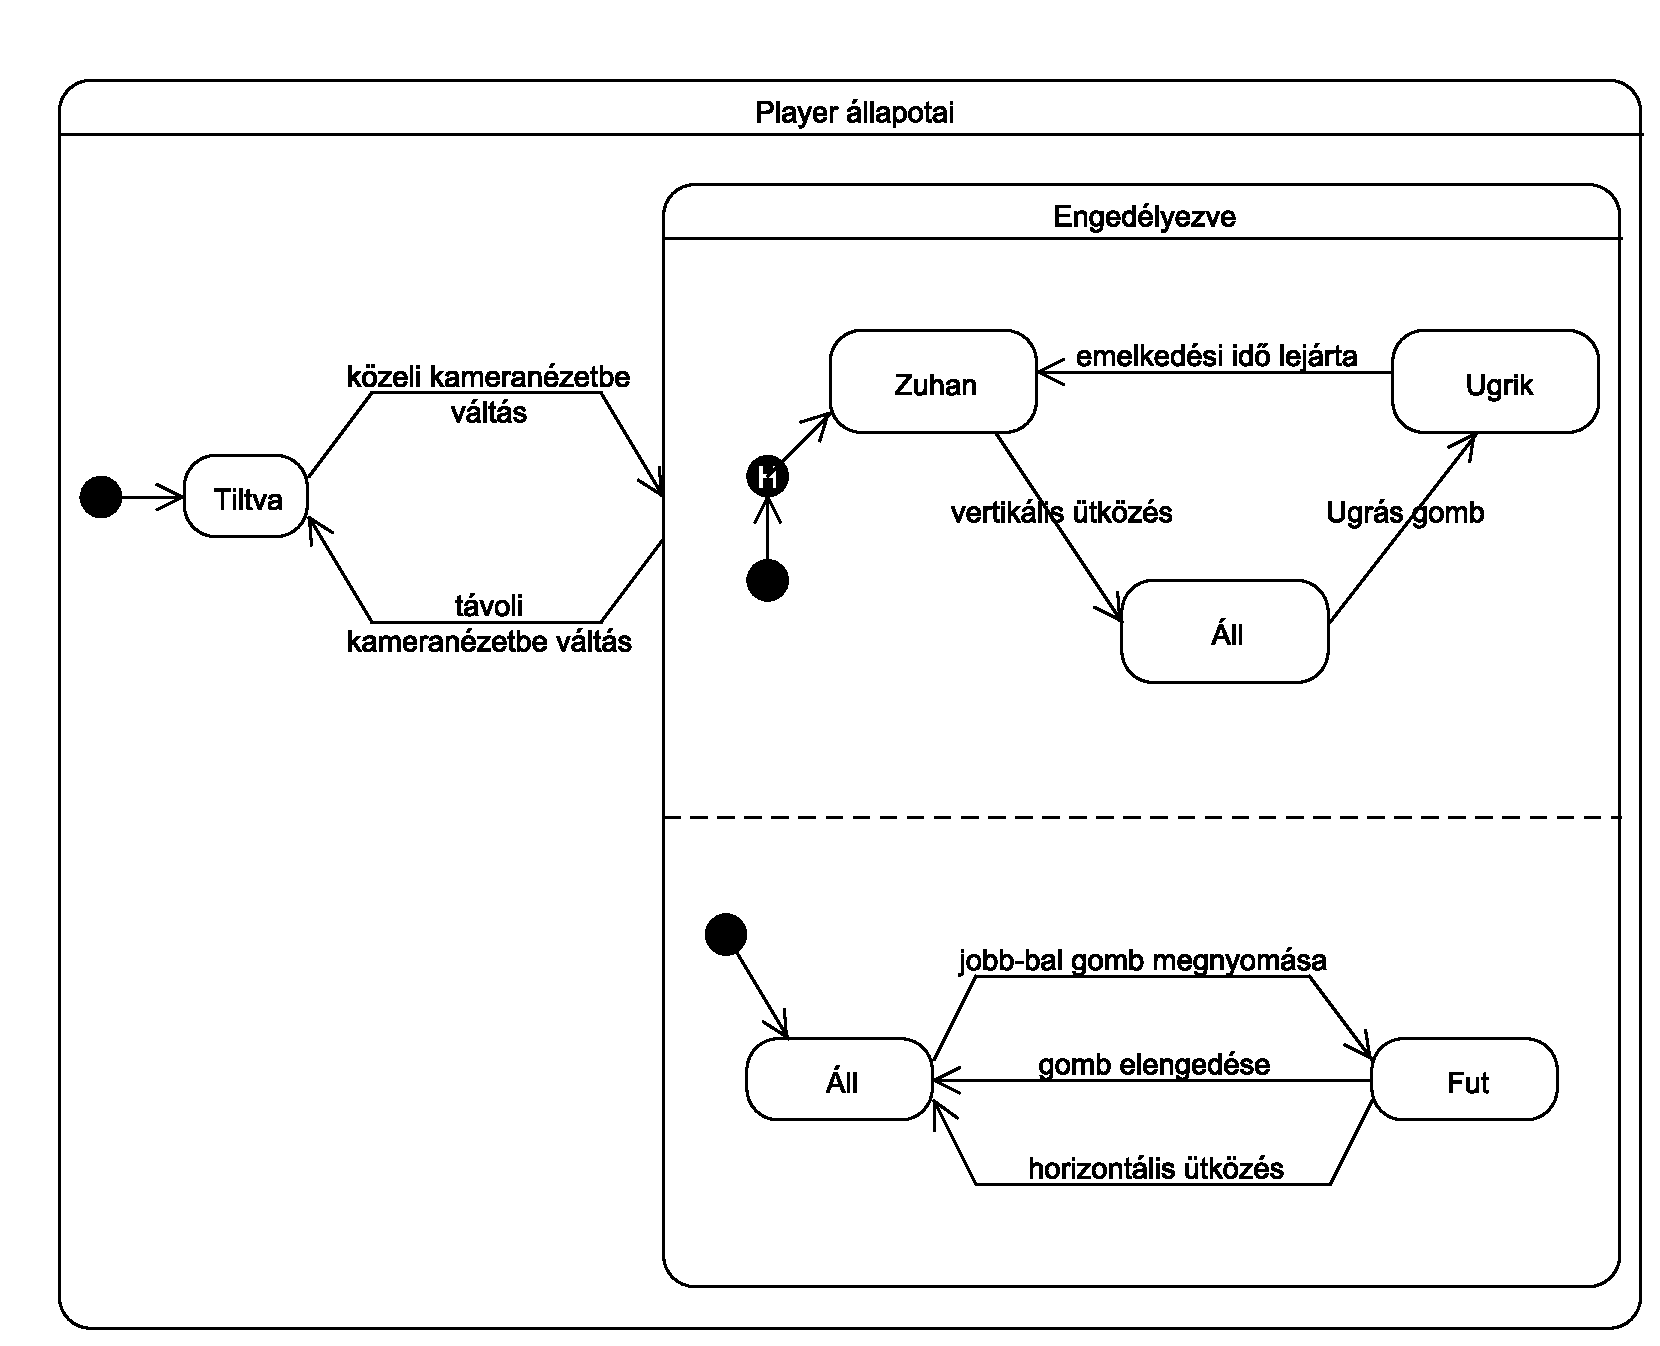
\includegraphics[scale=0.57]{03_statechart_Player.eps}

\newpage

\subsubsection{Level és KeyHolder osztály viselkedése}
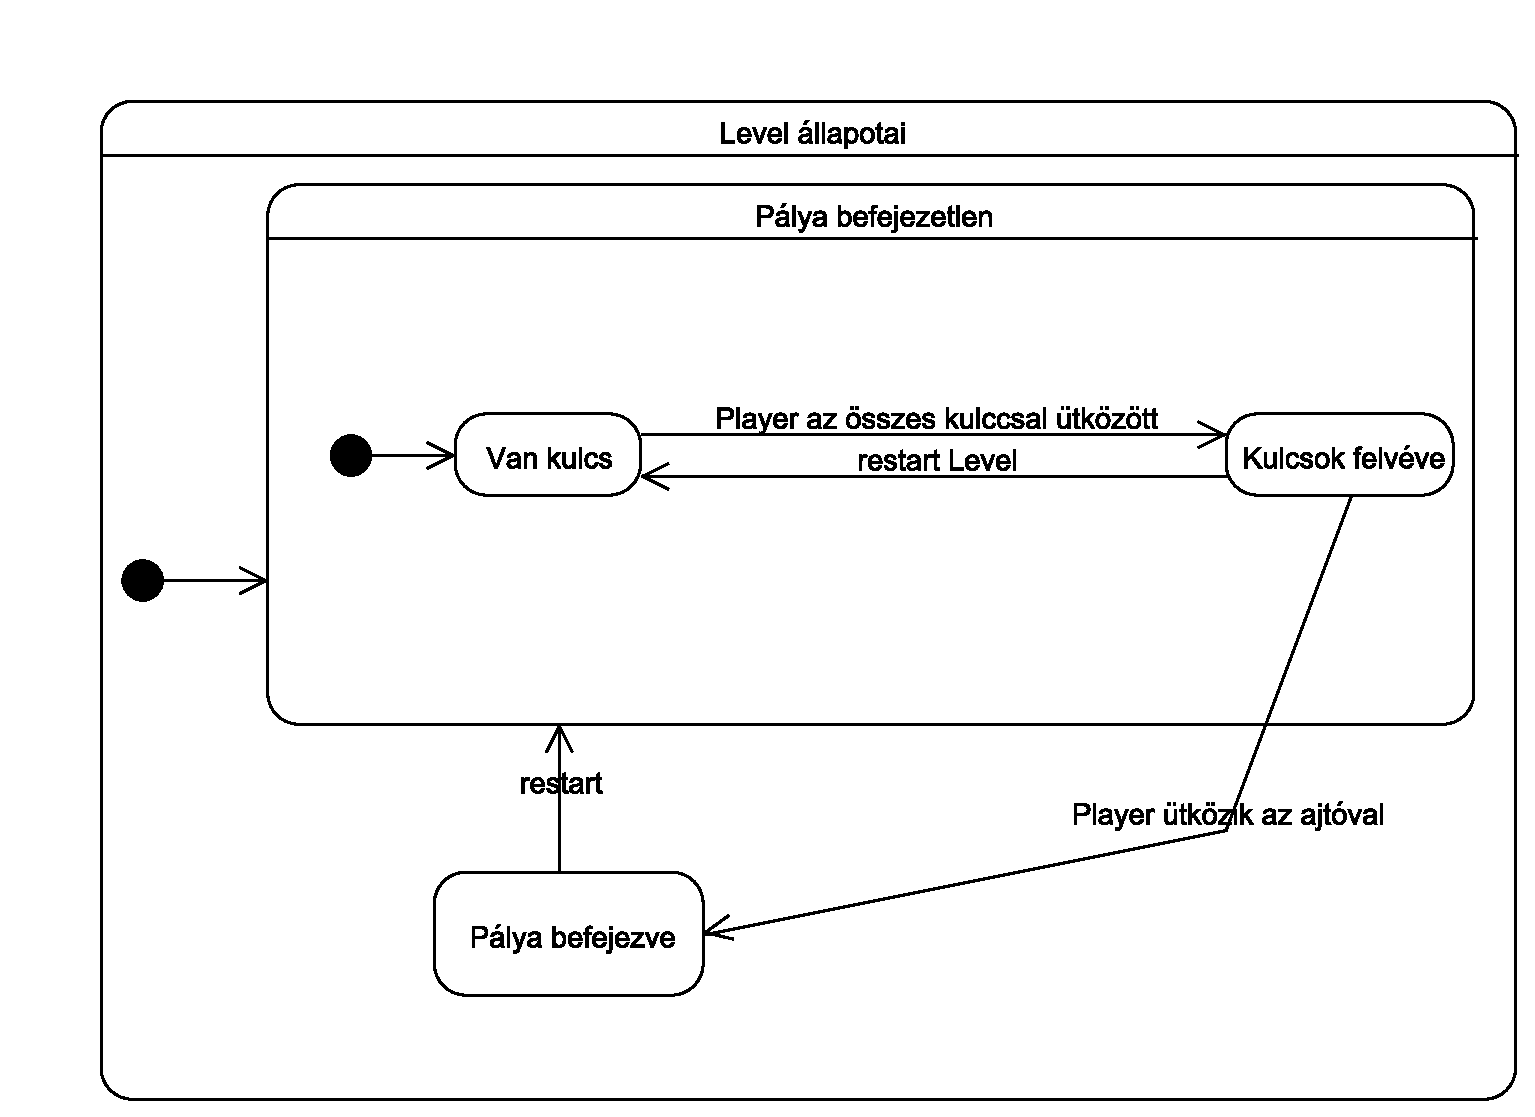
\includegraphics[scale=0.65]{03_statechart_Level2.eps}
\newpage
\subsection{Napló}

\begin{journal}

\journalentry{2012.02.21. 19:30}{2}{Biró}{\LaTeX{} fájlok formázása, újrarendszerezése}

\journalentry{2012.02.22. 12:30}{2}{Biró, Kanyó, Magyar, Tarjáni, Vajsz}{Személyes értekezlet. Feladatokat kiosztottuk, az analízis modell-beli főbb döntéseket meghoztuk. Osztálydiagram közös kidolgozása.}

\journalentry{2012.02.23. 16:45}{1,5}{Tarjáni}{Osztálydiagram Visual Studioban történő megrajzolása, közzététele.}

\journalentry{2012.02.23. 19:50}{1}{Vajsz}{Osztálydiagramot ellenőriztem, apróbb logikai hibákból adódó problémákat orvosoltam.}

\journalentry{2012.02.24. 13:00}{1,5}{Vajsz}{Nekikezdtem az eddigi megbeszéltek és az osztálydiagram alapján a szekvenciadiagram szerkesztésének majd elakadtam és észrevételeimet közöltem a csapattársakkal.}

\journalentry{2012.02.24. 19:00}{3,5}{Kanyó}{Objektumkatalógus elkezdése. Összes osztály informális leírása, kicsit finomabban mint a nyers megfogalmazás.}

\journalentry{2012.02.25. 10:00}{2,5}{Tarjáni}{Az objektumkatalógus kiegészítése, egyes helyeken módosítása}

\journalentry{2012.02.25. 11:00}{3}{Kanyó}{Osztályok formális leírásához sablon készítése, majd folyamatos feltöltése érdemi információval.}

\journalentry{2012.02.25. 12:45}{2,5}{Vajsz}{A válaszok és az újabb információk alapján a szekvenciadiagramon tovább dolgoztam majd újabb észrevételekkel és kérdéseikkel fordultam a csapattársaimhoz.}


\journalentry{2012.02.25. 11:00}{2}{Magyar}{UMLet szoftverrel való ismerkedés, osztálydiagram vizsgálata, state-chartok megtervezése}

\journalentry{2012.02.25. 13:40}{2}{Biró, Kanyó, Magyar, Tarjáni}{Személyes értekezlet. A PresentationCore-t kivettük az analízismodellből. A Player osztály újra lett tervezve. Szekvenciadiagrammok megtervezése.}

\journalentry{2012.02.25. 15:40}{2,5}{Kanyó}{Csináltam latex sablont az osztályok leírásához, elkészítettem két osztály formális leírását, javítottam UML hibákat.}

\journalentry{2012.02.25. 21:15}{0,5}{Vajsz}{A Game packagehez hiányzó class diagram adatait összegyűjtöttem, ezek alapján megszerkesztettem és pótoltam.}

\journalentry{2012.02.25. 22:00}{2,5}{Vajsz}{A rendelkezésre álló információkból megterveztem a játék inicializálását leíró szekvencia diagramot.}

\journalentry{2012.02.25. 23:15}{1}{Tarjáni}{Az osztályok formális leírásának folytatása}

\journalentry{2012.02.26. 00:45}{2,5}{Vajsz}{A 2012.02.25. 13:40-tól 15:40-ig tartó megbeszélés logfájlja alapján megterveztem további három szekvencia diagramot.}

\journalentry{2012.02.26. 03:00}{1,5}{Vajsz}{Megterveztem a player, azaz a mozgatható figura mozgásának szekvencia diagramját, valamint leellenőriztem az elmúlt 24 órában készült munkáimat.}

\journalentry{2012.02.26. 9:00}{4,5}{Kanyó}{Az osztályok formális leírásának folytatása}

\journalentry{2012.02.26. 10:30}{5}{Tarjáni}{Az osztályok formális leírásának befejezése}

\journalentry{2012.02.26. 10:00}{4,5}{Magyar} {State-chartok megírása, formázása, osztálydiagrammal való egyeztetése, state-chartok újraírása.}

\journalentry{2012.02.26. 17:15}{1,5}{Tarjáni}{Az első két fejezet ellenőrzése, hibák javítása}

\journalentry{2012.02.26. 20:00}{1}{Magyar}{Dokumentáció átolvasása, tagok feladatainak újraszinkronizálása}

\journalentry{2012.02.26. 21:00}{1}{Biró}{Dokumentáció átolvasása, javítási javaslatok felvetése, kisebb hibák orvoslása}

\journalentry{2012.02.26. 22:00}{3}{Magyar}{Szekvencia- és osztály diagramok átszerkesztése, naplóba képek beszúrása}

\journalentry{2012.02.27. 01:15}{2}{Magyar}{Osztály- és szekvencia-diagramok átdolgozása.}

\journalentry{2012.02.27. 03:15}{1}{Biró}{A state-chart sem maradt érintetlenül.}


\end{journal}

\end{document}